\documentclass[conference]{IEEEtran}
\IEEEoverridecommandlockouts
% The preceding line is only needed to identify funding in the first footnote. If that is unneeded, please comment it out.
\usepackage{cite}
\usepackage{amsmath,amssymb,amsfonts}
\usepackage{algorithmic}
\usepackage{graphicx}
\usepackage{textcomp}
\usepackage{xcolor}
\def\BibTeX{{\rm B\kern-.05em{\sc i\kern-.025em b}\kern-.08em
    T\kern-.1667em\lower.7ex\hbox{E}\kern-.125emX}}
\begin{document}

\title{Angle vs. Time vs. Strength vs. Mobility: Pros and Cons of different features for location verification}

%% author names commented out for initial release, might be needed later %%
%\author{
%    \IEEEauthorblockN{Somaye Hoseinpur}
%    \IEEEauthorblockA{\textit{Dept. of Computer Science} \\
%    \textit{University of Kaiserslautern}\\
%    Kaiserslautern, Germany \\
%    s\_hoseinpu19@cs.uni-kl.de}
%    \and
%    \IEEEauthorblockN{Sai Srinivas Jeevanandam}
%    \IEEEauthorblockA{\textit{Dept. of Computer Science} \\
%    \textit{University of Kaiserslautern}\\
%    Kaiserslautern, Germany \\
%    s\_jeevanan19@cs.uni-kl.de}
%    \and
%    \IEEEauthorblockN{Gabriele Monaco}
%    \IEEEauthorblockA{\textit{Dept. of Electronic and Information Technology} \\
%    \textit{University of Kaiserslautern}\\
%    Kaiserslautern, Germany \\
%    monaco@rhrk.uni-kl.de}
%}

\maketitle

\begin{abstract}
    Many applications are relying on location for various purposes in their activity, in general users need to advertise their own position to the server and can then spoof it. This can be dangerous in many contexts, from secure networks to aircraft. In this paper we are going to discuss about how to securely verify the location in wireless networks by exploiting physical properties of the incoming signals. It is indeed possible to determine, based on some measured parameters, if a location claim can be trustworthy and there are several methods how to do that. We are going through some of the physical properties that can be exploited for this purpose, pointing out advantages and disadvantages of the various approaches.
\end{abstract}

\section{Introduction}
Throughout this paper, we are going to discuss models in which a user needs to communicate its location to to the service handlers. We will refer as the former as \emph{prover}, since its job is to \emph{prove} its location, while the latter will be referred as \emph{verifier}, whose job is basically to check the prover's location. If not differently specified, all the communication happen in a wireless network, where the opponents can exchange radio messages.

In the next sections we will analyse separately each physical property: received angle, time of reception, signal strength, etc. For each of them we will point out strengths and weaknesses of the approach, to make clear in which application may them be effectively used and when they might not be a good option.

\section{Angle}
Angle of arrival or Direction of arrival can be used to estimate the location of a prover. The signal directions are considered as straight lines and the intersection of the several pairs of these lines indicate the location of the prover. AoA is detected with the help of i) using omni directional antennas ii) multiple static antenna arrays iii) Beamforming techniques. 
\begin{figure}[htp]
    \centering
    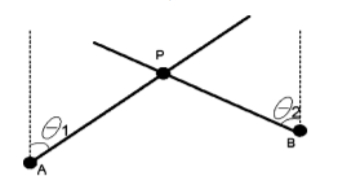
\includegraphics[width=4cm]{AoA.png}
    \caption{Angle of Arival \cite{angulation}}
    \label{fig:AoA}
\end{figure}
Once AoA is known Triangulation method can be used to find the location of the prover. Triangulation is a trigonometric approach where an unknown location is estimated based on two angles and distance between provers and verifiers. There are many limitations for location estimation based on AoA as discussed in next section. The major one is the presence of obstacles between prover and receiver. Many AoA based algorithms assume that there is a Line of Sight (LoS) between the nodes, which cannot be true in real world applications. So, there are algorithms which use help of other techniques along with AoA to do this. One of them is done using antenna arrays with array geometry and measuring differences in signal arrival times. Another method uses antenna arrays and RSSI ratios at each antenna to estimate AoA. Beamforming techniques are also used to shape the radiation pattern. 
A verification system verifies the calculated AoA with our estimated Angle. If these doesn’t match, then it means there is an attack. One advantage is that in general AoA is hard to forge by a single attacker so a distributed and a synchronized attack is required.

\begin{figure}[htp]
    \centering
    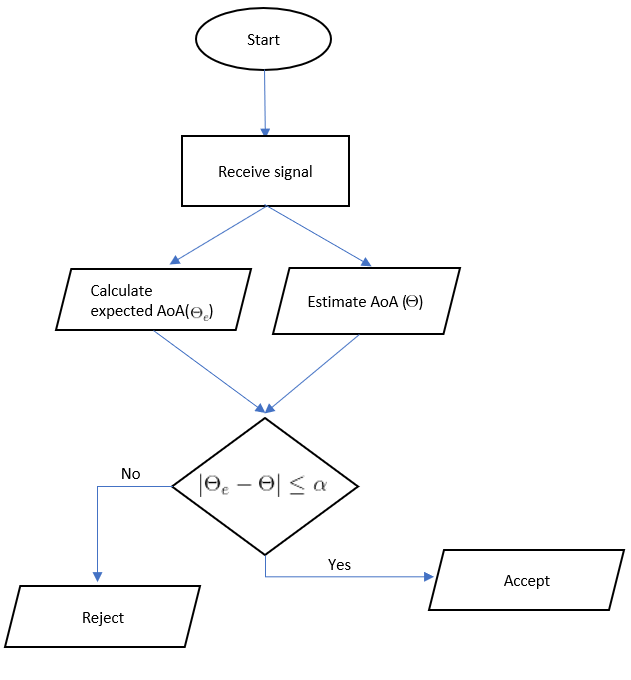
\includegraphics[width=7cm]{aoa_flow.png}
    \caption{Flow chart of a AoA based verification system \cite{abdelaziz19}}
    \label{fig:aoa_flow}
\end{figure}

As mentioned AoA based location techniques have limitations. The first and foremost being hardware dependencies i.e. for AoA to be directly measured extra hardware must be installed. Accuracy will also decrease as the distance increases between nodes. Another major drawback is that location estimation using AoA are susceptible to indoor multipath effects such as reflections, scattering, diffraction, refraction and absorption, especially in Non-Line of Sight (NLOS) conditions when shadowing occurs, this makes using these techniques in indoor conditions ineffective as it leads to erroneous measurements. A technique called fingerprinting is used to deal with multipath propagation situations. This method consists of two phases the offline phase and the online phase. In the offline phase a reference dataset is constructed by surveying signal characteristics at different know locations. In the online phase when the actual estimations is happening, measured data is compared with the reference dataset and estimation is achieved. But a major drawback for fingerprinting is that it is very labor intensive due to the offline phase, thus contributing to high deployment costs \cite{wielandt17}.

\section{Time}
%\section{Time}
Time is one of the several methods to verify the location of a node in the positioning systems. There are two different ways for obtain time measurement, which includes Time of Arrival (ToA) and Time Difference of Arrival (TDoA). These two techniques are widely used for detemining the position of a node or target.

\subsection{Time of Arrival (ToA)}

Usually an object at an unknown location is able to create signals at an unknown initial time. This signal can be detected by a set of sensor devices. Every sensor makes an estimation of the Time of Arrival of a signal. So, this method is based on the fact that when exactly the target sends a signal, the exact time the signal will be received by the sensor device and also the velocity of the signal \cite{brian17}.

\begin{figure}[htp]
    \centering
    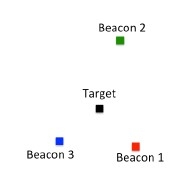
\includegraphics[width=3cm]{1.jpg}
    \caption{The location of Target and Beacons \cite{brian17}}
    \label{fig:Target location}
\end{figure}

In the following example, we have a target which surrounded by some Beacons. At time $t_1$ Beacon one sends a signal to the target, which the Target receives the signal at time $t_2$. Now the distance has to be calculated between the Target and Beacon one($d_1$). According to Fig. \ref{fig:Localization}, the next step is to draw a circle of possible location. The other two Beacons will send a signal to the target and then calculate the distance as the Beacon 1.

\begin{figure}[htp]
    \centering
    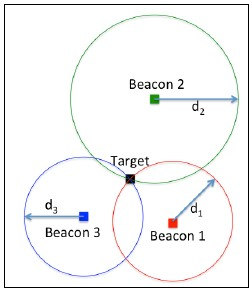
\includegraphics[width=2cm]{2.jpg}
    \caption{Localization \cite{jin18}}
    \label{fig:Localization}
\end{figure}

As mentioned before, the exact time of sending and receiving of a signal and the speed of signal (speed of light is considered) are requirements for calculating the distance.\cite{brian17}

Let the $t_s$ be the time which the emitter sends the signal and $t_a$ is the time which arrives to the target or target receives the signal. c is the speed of light.

Using this formula d (the distance) can be calculated and is used to determine the location of the target. ToA technique requires highly accurate synchronization of sender and receiver clocks \cite{jin18}

\begin{equation}
	\label{eqn:Localization}
    d = c \cdot (t_{arrival} - t_{sent})
\end{equation}
\eqncaption{Distance formula \cite{jin18}}

\subsection{Time Difference of Arrival (TDoA)}
Time Difference of Arrival technique which is also called multilateration which is often used in radar systems for localization of mobile targets \cite{schaefer15}. In this technique, three or more receivers at different locations capture the signal. The next step is the evaluation of the difference in arrival time of the signal. Because of the varying distances between transmitter and receivers, the signal arrives at different times for different receivers. The difference in arrival time is called TDoA \cite{brian17}.
For example, consider two Beacons (receivers) that received the signal at different points. Using this equation, we want to calculate the distance:

\begin{equation}
	\label{eqn:distance}
    \Delta d = c \cdot (\Delta t)
\end{equation}
\eqncaption{Distance formula \cite{jin18}}

Say c is the speed of light and $\Delta t$ is the difference in arrival times at different Beacons \cite{schaefer18}. Above mentioned equation is applicable to the two dimensions where $(x_1,y_1)$ and $(x_2,y_2)$ would be the positions of Beacons.

\begin{equation}
    \label{eqn:distance2}
    \Delta d = \sqrt{(x_2-x)^2-(y_2-y)^2} - \sqrt{(x_1-x)^2-(y_1-y)^2}
\end{equation}
\eqncaption{Distance formula for two dimension \cite{schaefer18}}


Consider $v_1$ and $v_2$ as synchronized versifiers (beacons in above example). The time of received signal is calculated using this equation:

\begin{equation}
    \label{eqn:time_received_sig}
    t_1 = t + \frac{\norm{p_1-p_P(t)}}{c}
    \quad \text{and} \quad
    t_2 = t + \frac{\norm{p_2-p_P(t)}}{c}
\end{equation}
\eqncaption{Time of received signal \cite{schaefer18}}

The Time Difference of Arrival will be calculated after collecting all the timestamps. Using this formula we wil have TDoA:


\begin{figure}[htp]
    \centering
    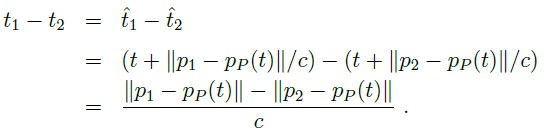
\includegraphics[width=8cm]{7.jpg}
    \caption{Calculating Time Difference of Arrival \cite{schaefer18}}
    \label{fig:formula}
\end{figure}
\begin{equation}
    \label{eqn:time_difference_arr}
    \begin{split}
        t_1 - t_2 \quad =& \quad t_1 - t_2 \\
        =& \quad (t+\frac{\norm{p_1-p_P(t)}}{c}) - (t+\frac{\norm{p_2-p_P(t)}}{c})\\
        =& \quad \frac{\norm{p_1-p_P(t)} - \norm{p_2-p_P(t)}}{c}
    \end{split}
\end{equation}
\eqncaption{Calculating Time Difference of Arrival \cite{schaefer18}}

In this equation only $p_p(t)$ has not given and it indicates the position of the Target! As you can see in the Fig. \ref{fig:hyp_location} the intersection of the different hyperbolas is the location of the $p_p(t)$ or the Target. \cite{brian17}

\begin{figure}[htp]
    \centering
    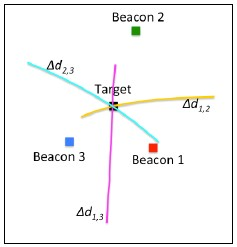
\includegraphics[width=4cm]{8.jpg}
    \caption{Possible location in relation to all Beacons \cite{brian17}}
    \label{fig:hyp_location}
\end{figure}

The more versifier (Beacon) we have, one extra hyperbola will be added which will also cross the $p_p(t)$ \cite{schaefer18}.

\subsection{Pro}
ToA technique does not need several information to estimate the location, this becomes one of the advantages of the ToA. The main advantage of the TDoA is that it does not require the communication between the emitter and the receiver. As there no communication in between, there would be no attacking to the system in order to identify the position of the Target. From a security prospective, this is a good point of the TDoA \cite{schaefer18}. Comparing to ToA, Time Difference of Arrival technique is quite beneficial due to requiring less computational power and also inexpensive and simple equipments.


\subsection{Cons}
The major disadvantage for the TDoA is the fact that it needs several measurements to calculate the location. In contrast, ToA does not require a lot of data to calculate the location. As a result, ToA technique need to synchronize the base station and mobile station in order to achieve the estimation of location without need for several information. One of the main weakness of TDoA systems is that it needs very accurate time synchronization which as a result, it makes this technique very expensive to adopt \cite{gante13}.

\subsection{Security Analysis}
Several protocols and approaches have been developed for detecting attacks on ToA and TDoA. However, before examining this approaches we have to know which kind of attack models could be occurred in such systems. Srdjan et al \cite{srivastava}have observed two kind of attacks: internal and external. Internal attacks are which an attacker can report a false position of a node. External attacks are able to convince both node and localization system that the node is not in its true position. These attacks could occur by reporting
false signal strengths and times of signal sending or receiving.

For example, consider Time Difference of Arrival systems which an attacker could be able to send signals to base stations at different times. This type of attack is in the category of Internal Attacks. Jamming is the type of attack that can occur in the system and is a type of External Attack. with jamming, the attacker can run timing attack that is possible with delaying the signal. An internal attack in the localization system could be also false position report. According to Srdjan et al's protocol, it is able to detect false position reports with checking the distance and also the regularity of the reported position \cite{srivastava}.

The most important privacy concern in TDoA Network is that, nodes reveal their location to any station that requests for a location verification. As a result, an attacker is able to send a location verification request to a node and know where exactly it is located \cite{srivastava}. As Srdjan et al stated, by using authentication is it possible to prevent such threats.


\section{Strength}
The strength of a received signal measured at the receiver's antenna is received signal strength (RSS). Two main factors that determine RSS i.e. transmission power, the distance between the transmitter. 
A Location Verification System (LVS) based on RSS is interesting because of following factors\cite{yan14}: i) RSS is measurable in a wireless system as this is part of the box. So, no extra hardware is required therefore complexity is less and less cost ii) Many standards and specifications such as 802.11b require RSS to be available. iii) Sometimes RSS might be the only reliable information. For example, non-line-of-sight environments. RSS is highly co-related to transmitter or provers location. Localization or location estimation algorithms which are based on RSS first calculate the distances to the prover. These are done with the help of multiple reference points which act as acceptors or verifiers. These distances can be calculated because there is an inverse square relation between received signal power and the distance. The following expression shows this\cite{pu11}
\begin{equation}
    P_r \propto \frac{1}{d^2}
    \label{gm_delay}
\end{equation}

Here P is the received power from a distance d. This expression gives us the path loss by comparing difference between transmitted and received power. In practical applications the variations of path loss can be highly dependent on the environment.

Once RSSI distance and path loss model is estimated, lateration techniques can be used find the exact position of the prover. Lateration techniques can be used to estimate the position based on multiple reference locations i.e. the distances from different reference locations can be considered as radius of circles with center as the reference location. The unknown location is the intersection of all these circles.

\begin{figure}[htp]
    \centering
    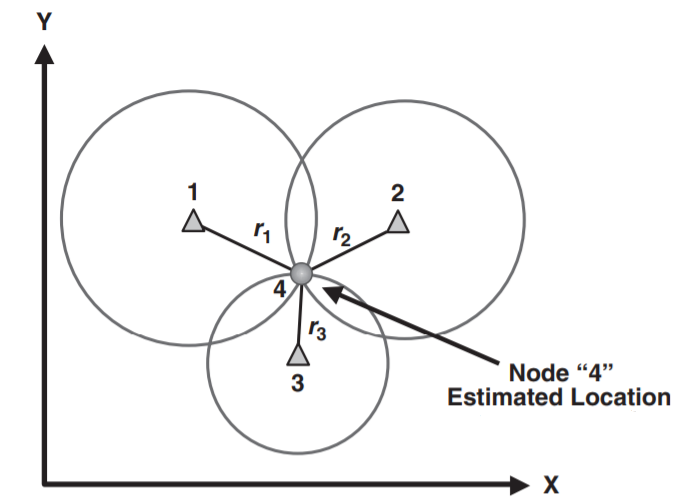
\includegraphics[width=7cm]{strength_trilat_pic.png}
    \caption{Location Estimation using Trilateration \cite{pu11}}
    \label{fig:strength_trilat_pic}
\end{figure}


\subsection{Limitations or disadvantages:} \label{rss_limitations}

Using RSS based location verification system is very tempting indeed because of the low cost, ready availability etc. as discussed above. But there are many limitations or problems. The main important problem is that the there is no control over transmit power. i.e. the attacker can act as a legitimate prover. So only weaker attackers can be detected. In the outdoor setting it is always advantageous to maintain the signal strength as high as possible to main a safety level of Link Quality Indicator, thus ensuring quality of our wireless communication. 
Another big limitation is that using such a system in an indoor environment is very hard. The main problems being multi path propagation, shadowing, and other noise sources makes location system based on RSS very hard to implement or in some cases completely unusable. 
\begin{figure}[htp]
    \centering
    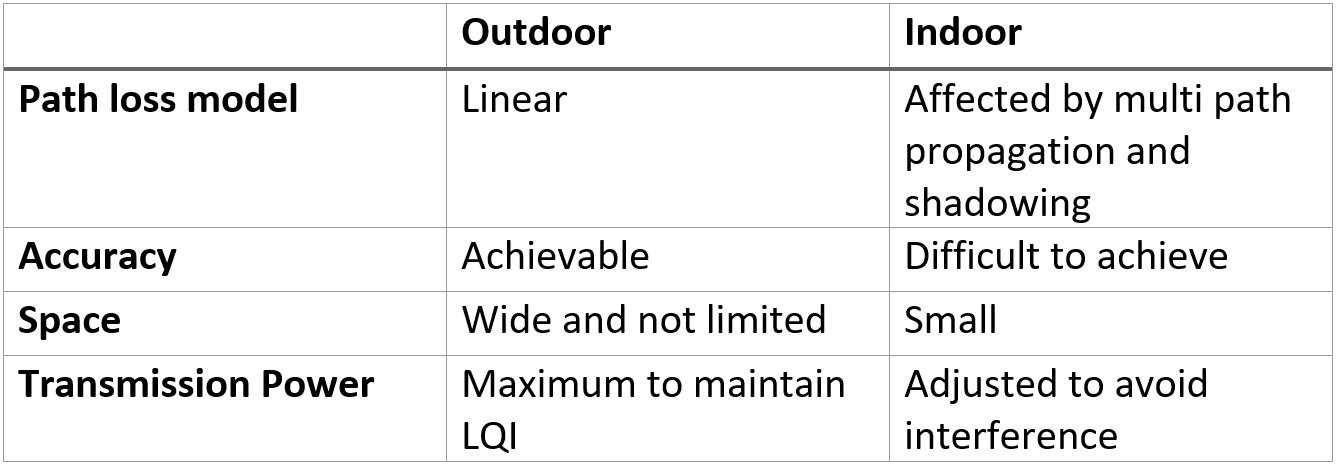
\includegraphics[width=9cm]{strength_comp_table.png}
    \caption{Outdoor vs Indoor \cite{pu11}}
    \label{fig:strength_comp_table}
\end{figure}
Finally, if mobility is involved i.e. if the wireless devices are mobile then an RSS base scheme alone becomes ineffective.


\subsection{Possible attacks and Current Methodologies} \label{rss_attacks}
RSS based systems are most vulnerable to spoofing attacks. Along with spoofing attackers try to use jamming and message replay to convince the verifiers.
There are different methods which try to detect spoofing and other attacks. Firstly, instead of using absolute signal strength Differential signal strength can be used. DRSS is difference between the signal strength values and the maximum value. In one of the detection mechanisms \cite{chenbook}, several access points (AP) at different fix locations are established which serve as sensors that measure RSS readings. A signalprint is constructed which is a vector of RSS at multiple access points. The idea is that signalprints are produced by wireless devices at different locations, which can be used to distinguish wireless devices located geographically apart. Different max and min matches and distributions are modelled based on which a RSS profile is established for each prover at different location. Any significant differences from these RSS patterns is considered as an attack. However, this method is computation intensive and when there is mobility involved it becomes ineffective.  Another verification method uses a set of covert base or verifiying stations. 

In coclusion RSS based location verification systems have many problems. These systems when combined with time difference of arrival (TDOA) perform better.




\section{Mobility}
In the following section we will discuss about the situation when the prover is moving, here some physical properties of the resulting signal may be exploited to verify it's actual location (or track, since many locations can be verified during time). We will talk about prover to reference either a moving object whose position (and movement) needs to be verified and an attacker who is not moving (speed vector = \(\vec{0}\)) and is trying to spoof its location. The prover is periodically sending location claims (sometimes referred as beacons) which are simple signals sent at a defined frequency. They contain information about the absolute position and absolute speed of the object, a timestamp of when the message has been sent is also included. Naturally, we are considering a potential attacker to be able to send any value in its messages, hence all the values contained in a claim need to be verified and cannot be trusted a priori. The verifiers are simple stationary receivers which are aware of their own position and which can exchange messages with one another (to verify claims in a distributed way, for instance), the attacker may know the verifiers positions and in general there's no limit in its knowledge.

\subsection{Mobility Differentiated Time of Arrival} \label{gm_sec_mtdoa}

When it comes to a moving prover, the principle of Time of Arrival (ToA) can be extended to Mobility-differentiated ToA (MDToA), according to this paradigm described in details in \cite{schaefer15}, over the time many beacons are collected from the prover, all of them containing informations about claimed position and speed. The verifier(s) can then compute according to a mathematical model the expected time of arrival of those messages (according to claimed parameters). If such a computation differs from the measured value, the verifier is able to detect a scam. Rather than \textit{location verification}, we can refer here as \textit{track verification}, since the prover is actually moving and we are going to verify its position over time, hence drawing a track.

In details, we define the propagation delay \(D_i\) as stated in formula \eqref{gm_delay}. Now we can say that the claim is trustworthy if the measured delay (\(D_{i,j}^m\)) between two beacons (here \textit{i} and \textit{j}) is equal to the claimed delay (obtained as difference of the claimed timestamps) plus the individual measured delays (see equation \eqref{gm_delay_trust} and figure \ref{gm_delay_pic}) \cite{schaefer15}.

\begin{equation}
    D_i = \frac{d_i}{c}
    \label{gm_delay}
\end{equation}
\emph{The time delay is obtained by dividing the absolute distance by the speed of light}

\begin{equation}
    D_{i,j}^m = D_{i,j} + (D_j - D_i)
    \label{gm_delay_trust}
\end{equation}

\begin{figure}
    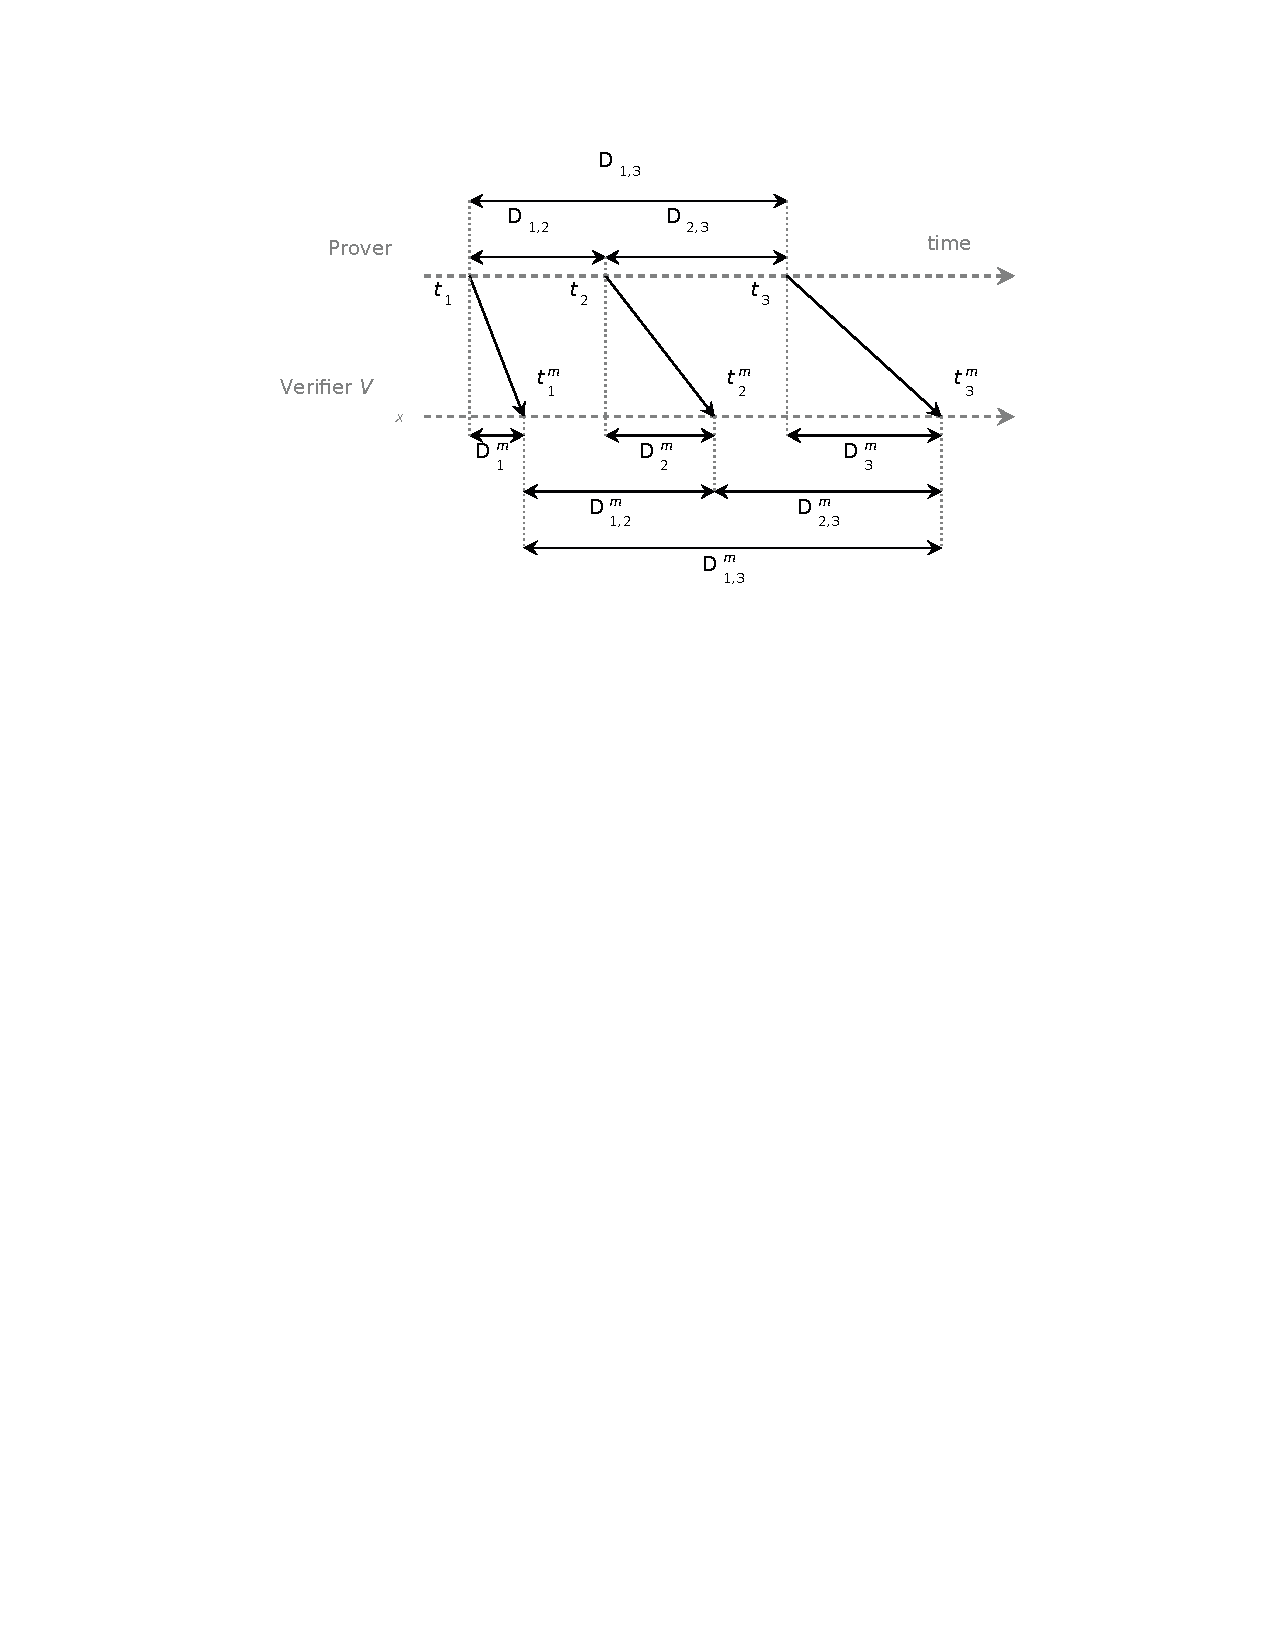
\includegraphics[width=.47\textwidth,trim={46mm 177mm 40mm 20mm},clip]{gm_delay_pic}
    \caption{Delays (noted as \textit{D}) over a timeline for three messages (\textit{1}, \textit{2} and \textit{3}) \cite{schaefer15}}
    \label{gm_delay_pic}
\end{figure}

\subsection{Frequency Difference of Arrival} \label{gm_sec_fdoa}

A similar approach can be used exploiting this phenomenon on a frequency domain, where it's known as \textit{Doppler effect}, the physical phenomenon according to which a wave signal (being it sound or light) emitted from one point, can be received with a different frequency if transmitter and receiver are moving relatively to each other (figure \ref{gm_doppler_base}). Indeed depending on direction and speed of the transmitter (here the prover), a specific frequency shift would be measured by the receiver (here the verifier). In an analogous way with respect to the MDToA, a set of equations can be derived from receiver location (known), sender location and speed (both claimed), by means of those is possible to intercept unexpected behaviours. We will refer to this principle as Frequency Difference of Arrival (FDoA) \cite{schaefer16} \cite{ghose15}. The law that must be satisfied by the prover is reported in equations \eqref{gm_radspeed} and \eqref{gm_doppler}.

\begin{equation}
    \label{gm_radspeed}
    v_x = \vec{v} \cdot cos\theta
\end{equation}
\emph{\(v_x\) is the radial speed, which is the component of the prover's speed directed to the verifier. Here \(\theta\) is the angle between the vector \(\vec{v}\) and the verifier position as can be seen in figure \ref{gm_doppler_spd}}

\begin{equation}
    f_m = \frac{f_0}{1-\frac{v_x}{c}}
    \label{gm_doppler}
\end{equation}

\begin{figure}
    \begin{center}
        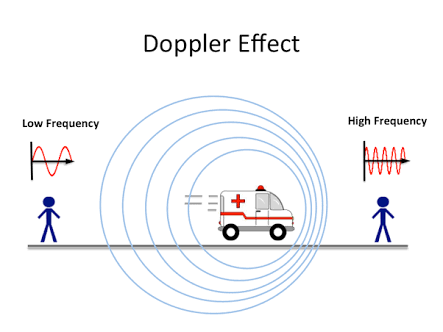
\includegraphics[width=.37\textwidth]{gm_doppler_base.png}
        \caption{The Doppler effect as can be seen considering a sound wave, the same phenomenon happens when dealing with light radiations \cite{dopplersrc}}
        \label{gm_doppler_base}
    \end{center}
\end{figure}

\begin{figure}
    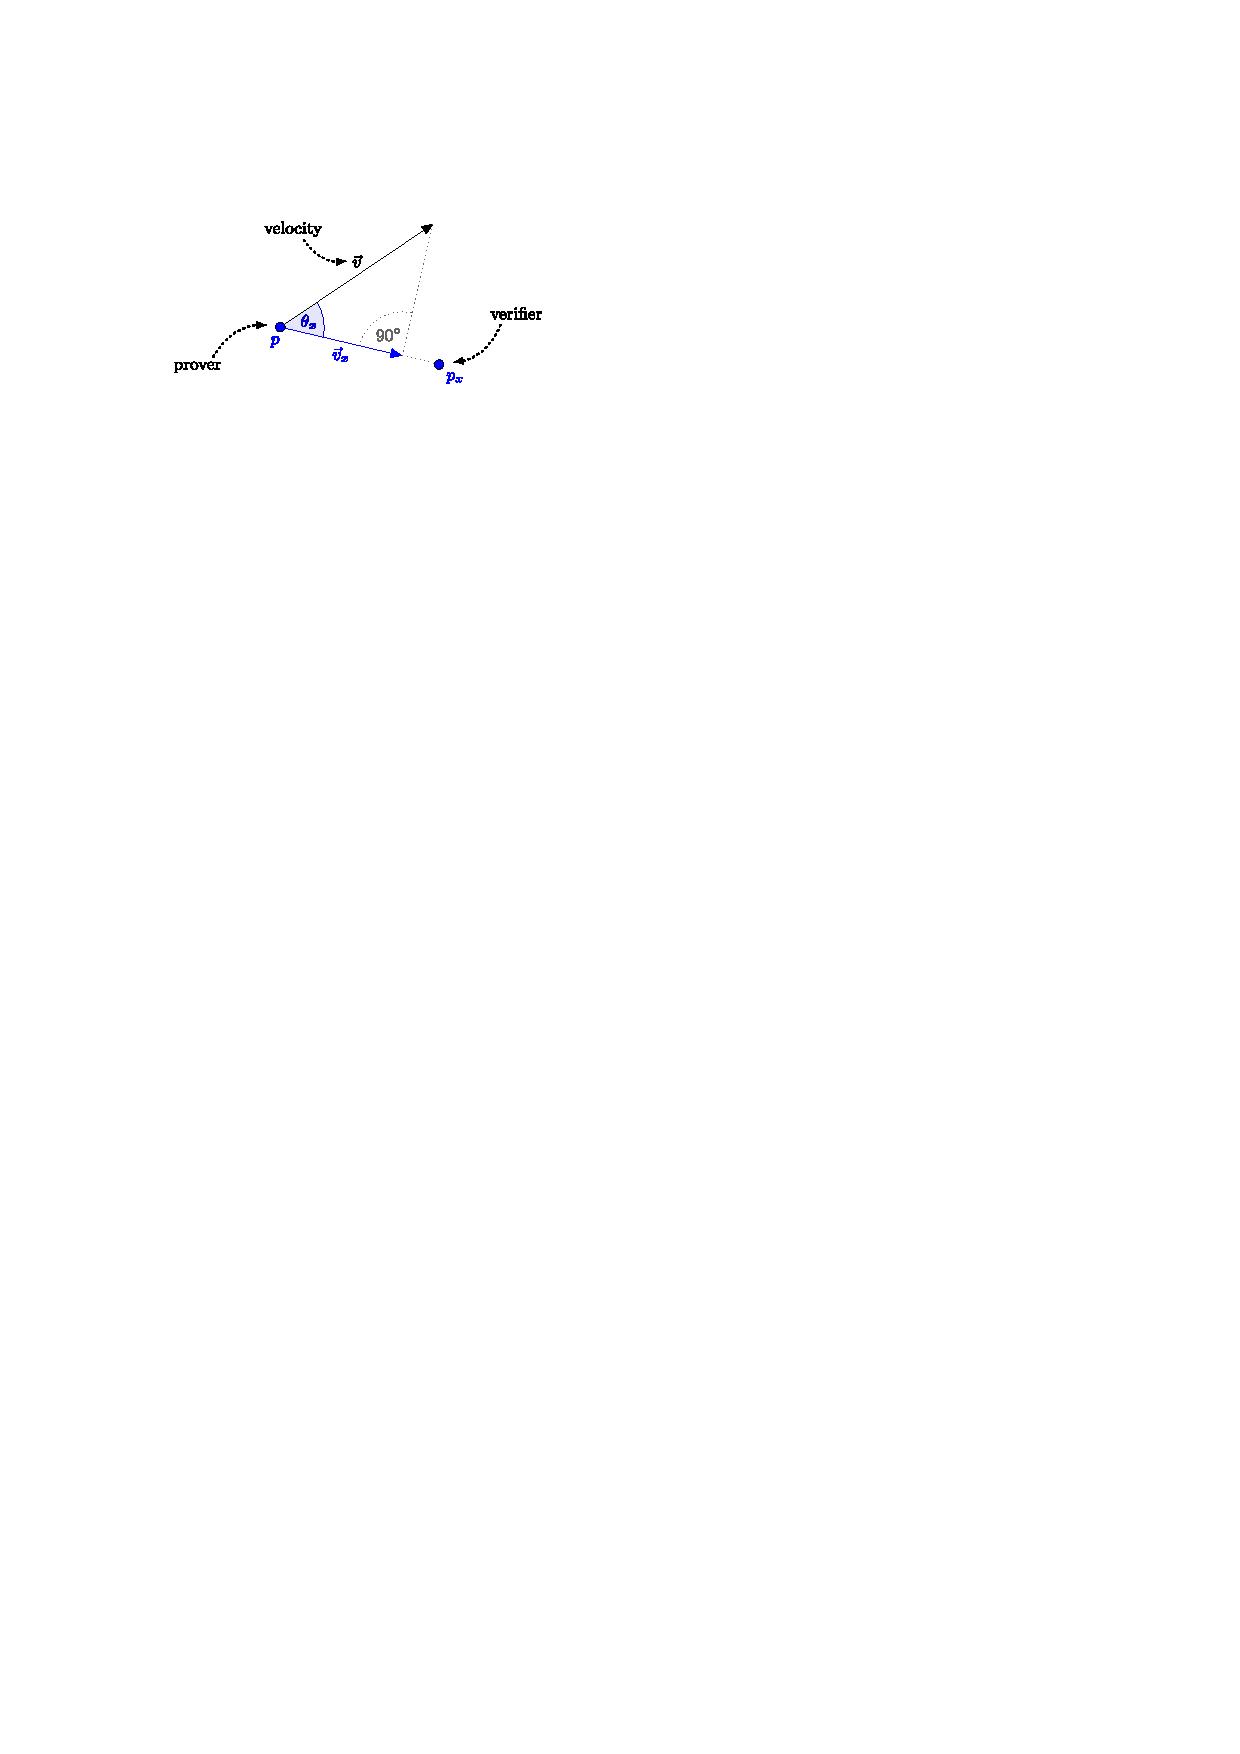
\includegraphics[width=.47\textwidth,trim={27mm 230mm 115mm 35mm},clip]{gm_doppler_spd}
    \caption{Relative speed component used to compute the Doppler effect \cite{schaefer16}}
    \label{gm_doppler_spd}
\end{figure}

The verification process, as stated in \cite{schaefer16} and \cite{ghose15}, is carried out by checking the measured frequency \(f_m\) on different location claims against the provided speed and the initial expected frequency. As the formulas are pointing out, we cannot really check the location, since we are only analysing the speed vector, this approach can then be defined as \textit{Motion Verification}. We can then just be sure if the prover is moving as claimed, with respect to our verifier, regardless on it's actual location.

\subsection{Possible attacks and how to cope with them} \label{gm_sec_attacks}

While defining both MDToA and FDoA we described a model with one verifier and one prover. In case the prover was actually malicious, we didn't consider it to be aware of the verification system and hence we are not considering it to be able to take any counter measure. Instead it can be proven that, by properly adjusting the delay while sending messages, an attacker can mock it's location and still fulfil the verifier's requirements (\cite{schaefer15} and \cite{schaefer16}).

For instance considering the MDToA case, we suppose an attacker to dispose of a single antenna to transmit its location claims, such attacker would be able to simply add the proper delay while sending beacons and change timestamp on them accordingly (in equation \eqref{gm_delay_trust} we relied on those values) to properly mock it's location to the verifier.

Schäfer et al. \cite{schaefer15} demonstrated that, with the same attacker model involving a single transmitter broadcasting to all the verifiers, simply adding one more verifier is reducing by one degree of freedom the claims the prover can mock. Indeed, while considering the case with a single verifier, the attacker could adjust transmission times and timestamps to virtually mock any track. Instead, by simply adding a new verifier, only some tracks can be successfully spoofed, using the same constructed delays, for both of them.

This trivial modification is drastically improving security, since now the two verifiers can spot suspicious tracks, which may even become unlikely or impossible in some use cases (where the prover is bound to some specific tracks). It is then straightforward to further improve this solution by adding another verifier, which would restrict the usable track by another degree of freedom, a fourth verifier would theoretically even reduce the available track to a single point, which would not be feasible for a mobile prover.
While in theory a set of four verifiers is enough to track down a malicious prover, some additional verifiers may be required in practice to avoid some noise interferences.

A similar conclusion may be derived from the Doppler shift method (as in \cite{schaefer16} and \cite{ghose15}: in this case, the attacker may adapt its transmission frequency to mock the signal for a single verifier, but the addition of more receivers can again reduce the attacker's freedom and eventually make it impossible for a malicious claim to remain undetected, if the verifiers are well placed (e.g. not aligned with each other).

The previously adopted countermeasures only hold under the assumption of an attacker who can use a single transmitter for every verifier, see section \ref{gm_sec_cons} for further details.

\subsection{Methods in action: Air Traffic Monitoring} \label{gm_sec_adsb}

A typical use case of those methods may be aircraft tracking, at the time of writing (2020) the new standard system for locating aircraft, the Automatic Dependent Surveillance-Broadcast (ADS-B), is about to be officially operating to manage air traffic. According to the ADS-B protocol (\cite{adsb}), the airplanes are supposed to know their current parameters (position, speed, etc..) via external systems such as GPS and they are periodically broadcasting such data. Control centers are, instead, gathering all the data related to air traffic and can then control it accordingly. This protocol is expected to be a replacement for classical radar based systems, its implementation is way cheaper and it can be more accurate, but it hasn't been designed with security in mind. Indeed there's no way to verify if received ADS-B packets can be trusted or not.
Costin et al. \cite{costin12} proved that it's not just feasible, but it's also easy with highly available equipments and software, this means that potentially anybody may be able to spoof signals of thousands of \textit{ghost} aircraft, thus making impossible for an airport control center to work and causing severe problems or even danger among real airplanes.

Both MDToA and FDoA can be really helpful in this situation as they both don't require any change on hardware devices on aircraft or in the protocol itself, which is a key feature especially in this field, where a change in protocol may require a full fleet upgrade, which likely would need two decades to become effective (ADS-B has been proposed in the 90s). Indeed those location verification checks are significantly enhancing security by simply exploiting physical properties of the transmission medium, the same control centers reading ADS-B beacons, which are already trusted, can directly be upgraded to also verify the locations of those messages, thus making the solution cheap as well. By exploiting time or frequency \textit{difference} there's even no need to keep time synchronization among verifiers and moreover both the solutions are robust since they are proven to be secure with a certain number of verifiers.

\subsection{Weaknesses and limitations} \label{gm_sec_cons}
As stated earlier, FDoA cannot be used for Track verification but rather for Motion verification, that means that we could spot a malicious attacker only if its speed vector is behaving as expected over time. In this way it can work perfectly against steady attackers, but if also the attacker can move it might be able to successfully spoof its signals. That is however not likely in many applications, since the attacker may need to have a very high speed or to travel along very specific tracks. Besides that, in practice FDoA can be heavily affected by noise in signals, it hence needs a deeper and more refined approach as pointed out by Schäfer et al. \cite{schaefer16}, with their approach analysing multiple location claims can drop to zero the detection error rate.

In addition, Schäfer et al. \cite{schaefer15} suggest that even MDToA can perform worse than expected in real world: it's not guaranteed that all verifiers clocks run with the same speed and their difference might not result as negligible for this purpose. Hence all the errors must be taken into account and the actual performance may be less accurate than expected.

The main limitation of both the methods is related to the fact that we are supposing the verifier to be able to transmit from a single position. Instead, if the attacker could use multiple transmitters, even one for each verifier, and if it could tune the transmission power to avoid all the verifiers to be able to listen to more than one transmitter, it could virtually be able to adjust delays and frequencies separately for each of them. In this way it would be simply impossible to detect the scam and the attacker would be able to spoof any possible position. By all means, that would be a tremendously resource demanding solution, since it would involve many transmitters, properly located and we can assume our attacker model would not reach this depth. It is not likely for the attacker to precisely know all the verifiers position and their reception range, by missing this knowledge it wouldn't be possible to carry on with such a solution.



\section{Conclusion}
In this article, we gave a general overview of the different location verification techniques. These mechanisms have been an important subject for conducting study and research for positioning systems. However, they have to be considered from different aspects specially security. Because they can be used in applications such as IoT and any systems that require positioning objects. So improving these techniques will result in better positioning. We studied and analyzed the advantages and disadvantages of these techniques. To come to a conclusion, considering the project for positioning systems one of these techniques of mixed of them can be used. 
As mentioned before, RSS based location verification systems have many problems. These systems when combined with time difference of arrival (TDOA) perform better. Both ToA and TDoA systems are widely used for to get location in the navigation systems. However, as mentioned before an attacker could easily detect the position of a node in the ToA network, so it is recommended to obtain TDoA technique.Considering the big geolocation systems, two factors seem to be more important which are security and accuracy. Although AoA based localization techniques are not widely implemented they can be used to increase accuracy and improve verification by using along with other features. Right now even tough RSS based systems provide good enough solutions to many present applications there are limitations, challenging requirements which needs to be addressed.
In developing positioning systems, the Prioritization should be considered. As in some systems less accuracy leads to undesirable results and similarly some systems prefer the higher security. Therefore, choosing between two techniques needs to know the preferences first. All in all, four mechanisms can be compared in many aspects but depending on the application area, one technique can be chosen. Nevertheless, by advancing the technology it is expected that these techniques or even a brand new technique could be developed that has a better security and precision.

\begin{thebibliography}{00}

\bibitem{angulation} ANGULATION. http://kom.aau.dk/group/10gr891/methods/Triangulation/Angulation/ANGULATION.pdf/ [Accessed: January 2020]
\bibitem{abdelaziz19} A. Abdelaziz, R. Burton, F. Barickman, J. Martin, J. Weston and C. E. Koksal, "Enhanced Authentication Based on Angle of Signal Arrivals," in IEEE Transactions on Vehicular Technology, vol. 68, no. 5, pp. 4602-4614, May 2019.
\bibitem{wielandt17} Wielandt, S.; Strycker, L.D. Indoor Multipath Assisted Angle of Arrival Localization. Sensors 2017, 17, 2522.
\bibitem{schaefer15} M. Schäfer, V. Lenders and J. Schmitt ``Secure Track Verification,'' 2015 IEEE Symposium on Security and Privacy, San Jose, CA, pp. 199-213, 2015.
\bibitem{schaefer16} M. Schäfer, P. Leu, V. Lenders and J. Schmitt ``Secure Motion Verification using the Doppler Effect,'' Proceedings of the 9th ACM Conference on Security \& Privacy in Wireless and Mobile Networks, pp. 135-145, 2016.
\bibitem{ghose15} N. Ghose and L. Lazos ``Verifying ADS-B navigation information through Doppler shift measurements,'' 2015 IEEE/AIAA 34th Digital Avionics Systems Conference (DASC), pp. 4A2-1, 2015.
\bibitem{costin12} A. Costin and A. Francillon ``Ghost in the Air (Traffic): On insecurity of ADS-B protocol and practical attacks on ADS-B devices,'' Black Hat USA, pp.1-12, 2012.
\bibitem{brian17}B. Keefe ``Finding Location with Time of Arrival and Time Difference of Arrival Techniques.'' ECE Senior Capstone Project (2017).
\bibitem{jin18}Jin, Bonan, Xiaosu Xu, and Tao Zhang. ``Robust time-difference-of-arrival (TDOA) localization using weighted least squares with cone tangent plane constraint.'' Sensors 18.3 (2018): 778.
\bibitem{schaefer18}M. Schaefer ``Mobility Improves the Security of Location Awareness in Wireless Networks.'' (2018).
\bibitem{gante13}D. Gante, Alejandro, M. Siller. ``A survey of hybrid schemes for location estimation in wireless sensor networks.'' Procedia Technology 7 (2013): 377-383.
\bibitem{adsb}ADS-B Info. https://www.ads-binfo.com/. [Accessed: January 2020]
\bibitem{dopplersrc}INSIGHT. https://www.insightsonindia.com/2016/03/01/insights-daily-current-events-01-march-2016/ [Accessed: January 2020]
\bibitem{srivastava}R. Kasper, M. Srivastava. ``Secure location verification with hidden and mobile base stations.'' IEEE Transactions on Mobile Computing 7.4 (2008): 470-483.
\bibitem{yan14} S. Yan, R. Malaney, I. Nevat and G. W. Peters, "Signal strength based wireless Location Verification under spatially correlated shadowing," 2014 IEEE International Conference on Communications (ICC), Sydney, NSW, 2014, pp. 2617-2623.
\bibitem{pu11} Pu, Chuan Chin \& Pu, Chuan-Hsian \& Lee, Hoon-Jae. (2011). Indoor Location Tracking Using Received Signal Strength Indicator. 10.5772/10518. 
\bibitem{chenbook} Yingying Chen, Jie Yang, Chapter 8 - Defending Against Identity-Based Attacks in Wireless Networks, Handbook on Securing Cyber-Physical Critical Infrastructure, Morgan Kaufmann,2012, Pages 191-222

\end{thebibliography}

\end{document}
